\begin{exercise}{Maison au bord du lac}{3}{Sup, spé}
{Thermodynamique,machines thermiques,pompe à chaleur}{lelay}

On considère un bûcheron (fin)landais habitant une maison au bord d'un lac près la mer du Nord. L'eau du lac est à 5 degrés Celsius, l'air ambiant est à $-10$ degrés Celsius. Le but de cet exercice est de déterminer si le bûcheron arrivera à chauffer sa maison à 20 degrés (sans utiliser de bois !).

\begin{questions}
    \questioncours Principes thermodynamiques appliqués aux machines thermqiues, rendement de Carnot.
    \question Faire un schéma, incluant des petits poissons dans le lac, des oiseaux dans le ciel et un chat dans la maison du bûcheron.
    \question Le bûcheron souhaite chauffer sa maison. Peut-il y arriver sans utiliser le lac ?
    \question Montrer que le bûcheron peut se servir d'une machine thermique pour générer du travail. Comment alors utiliser ce travail pour chauffer sa maison ? Quelle est l'entropie créée par ce procédé ?
    \question Le bûcheron (qui est un peu excentrique) souhaite en fait se chauffer de manière isentropique. Comment faire ?
    \question Définir et calculer l'efficacité de ce procédé selon la méthode utilisée.
    \question Retrouver le résultat grâce à une méthode plus simple
\end{questions}

\end{exercise}

\begin{solution}
\begin{questions}
    \questioncours Principes thermodynamiques appliqués aux machines thermiques, rendement de Carnot.
    \question 
\begin{center}
    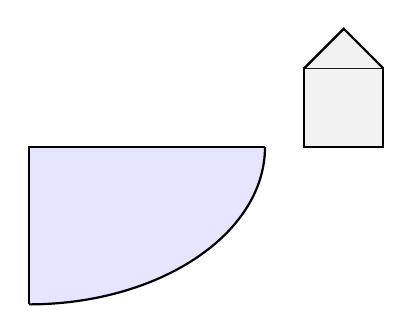
\begin{tikzpicture}
    \tikzset{
    partial ellipse/.style args={#1:#2:#3}{
        insert path={+ (#1:#3) arc (#1:#2:#3)}
    }
    }
    \fill[fill=blue!10] (0,0) -- (0,-2) -- (3,0);
    \filldraw[thick, color=black, fill=blue!10] (0,0) [partial ellipse=-90:0:3 and 2];
    \draw[black, thick] (0,-2) -- (0,0) -- (3,0);
    
    \filldraw[color=black, thick, fill=black!5] (3.5,0) rectangle (4.5,1);
    \filldraw[color=black, thick, fill=black!5] (3.5,1) -- (4,1.5) -- (4.5,1);
    
    \end{tikzpicture}
\end{center}
    \question Non, à cause du second principe.
    \question Il fait une machine thermique entre le lac et l'air, générant un travail $W$. Il peut convertir ce travail par exemple avec ue résistance chauffante. L'entropie produite est alors $W/T$ avec $T$ la température de la maison.
    \question Il branche la machine thermique de la question précédente sur une autre machine thermique chauffante isentropique. La source chaude est alors la maison et la source froide est soit l'air (moins efficace car plus froid, mais permet d'utiliser de l'énergie pas chère puisqu'on s'en fout de le refroidir) soit le lac (plus efficace, mais on refroidit plus le lac). 
    \question L'air on s'en fiche, on veut optimiser $Q$ le transfert thermique à la maison par rapport à $Q_\ell$ le transfert thermique au lac (pour ne pas le faire geler). On trouve 
    \begin{align*}
        \frac{Q}{Q_\ell} &= \frac{T_\ell - T_a}{T - T_\ell}\frac{T}{T_\ell}
    \end{align*}
    \question Utiliser une machine tritherme ne générant pas de travail.
\end{questions}
\end{solution}